% UTF-8 encoding
% Compile with latex+dvipdfmx, pdflatex, xelatex or lualatex

\documentclass[hyperref, UTF8]{ctexart}
\usepackage{amssymb}
\usepackage{amsmath}
\usepackage{graphicx}
\usepackage{subfigure}
\usepackage{geometry}
\usepackage{caption}
\usepackage{upgreek}
\newcommand{\under}[1]{\frac{1}{#1}}
\newcommand{\underpone}[1]{\frac{#1}{1+#1}}
\newcommand{\volt}{{\rm V}}
\newcommand{\source}{{\rm S}}
\newcommand{\second}{{\rm s}}
\newcommand{\radian}{{\rm rad}}
\newcommand{\ampere}{{\rm A}}
\newcommand{\milliampere}{{\rm mA}}
\newcommand{\microampere}{{\rm \upmu A}}
\newcommand{\decibel}{{\rm dB}}
\newcommand{\hertz}{{\rm Hz}}
\newcommand{\kilohertz}{{\rm kHz}}
\newcommand{\megahertz}{{\rm MHz}}
\newcommand{\gigahertz}{{\rm GHz}}
\newcommand{\ohm}{\Omega}
\newcommand{\kiloohm}{{\rm k}\Omega}
\newcommand{\watt}{{\rm W}}
\newcommand{\kilowatt}{{\rm kW}}
\newcommand{\degree}{^{\circ}}
\newcommand{\farad}{{\rm F}}
\newcommand{\microfarad}{{\rm \upmu F}}
\newcommand{\millifarad}{{\rm mF}}
\newcommand{\henry}{{\rm H}}
\newcommand{\J}{{\rm j}}
\newcommand{\D}{{\rm d}}
\newcommand{\E}{{\rm e}}

\title{电子学基础——第十二次作业}
\author{LXQ}
\date{2019.12.26}

\geometry{left=2.0cm, right=2.0cm, top=2.5cm, bottom=2.5cm}
\linespread{1}

\begin{document}

\maketitle

\paragraph{12.1} \label{12.1}
    Determine the transfer function, $Y/X$, for the systems shown in Fig. 12-77.
    \begin{figure}[!htb]
        \centering
        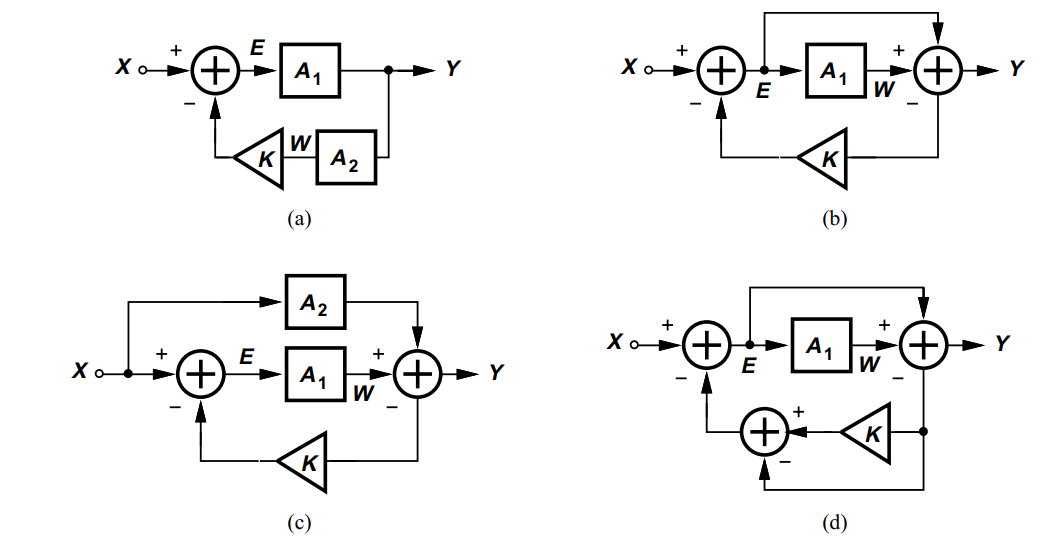
\includegraphics[width=0.701\textwidth]{p12-77.png}
        \caption*{Figure 12-77}
    \end{figure}        
\paragraph{解}
    (a) 
    \begin{gather*} \left\{ \begin{aligned}
        E & = X - EA_1A_2K \\
        Y & = EA_1
    \end{aligned} \right. \end{gather*}
    $$\therefore \frac{Y}{X} = \frac{A_1}{1+A_1A_2K}$$

    (b)
    \begin{gather*} \left\{ \begin{aligned}
        E & = X - (EA_1-E)K \\
        Y & = EA_1 - E
    \end{aligned} \right. \end{gather*}
    $$\therefore \frac{Y}{X} = \frac{A_1-1}{1+(A_1-1)K}$$

    (c)
    \begin{gather*} \left\{ \begin{aligned}
        E & = X - (EA_1 - A_2X)K \\
        Y & = EA_1 - A_2X 
    \end{aligned} \right. \end{gather*}
    $$\therefore \frac{Y}{X} = \frac{A_1 - A_2}{1+A_1K}$$

    (d)
    \begin{gather*} \left\{ \begin{aligned}
        E & = X - [(EA_1 - E)K - (EA_1 - E)] \\
        Y & = EA_1 - E
    \end{aligned} \right. \end{gather*}
    $$\therefore \frac{Y}{X} = \frac{A_1-1}{1+(K-1)(A_1-1)}$$
\paragraph{12.4} \label{12.4}
    Calculate the loop gain of the circuits illustrated in Fig. 12-78. Assume the op amp exhibits an open-loop gain of $A_1$, but is otherwise ideal. Also $\lambda = 0$.
    \begin{figure}[!htb]
        \centering
        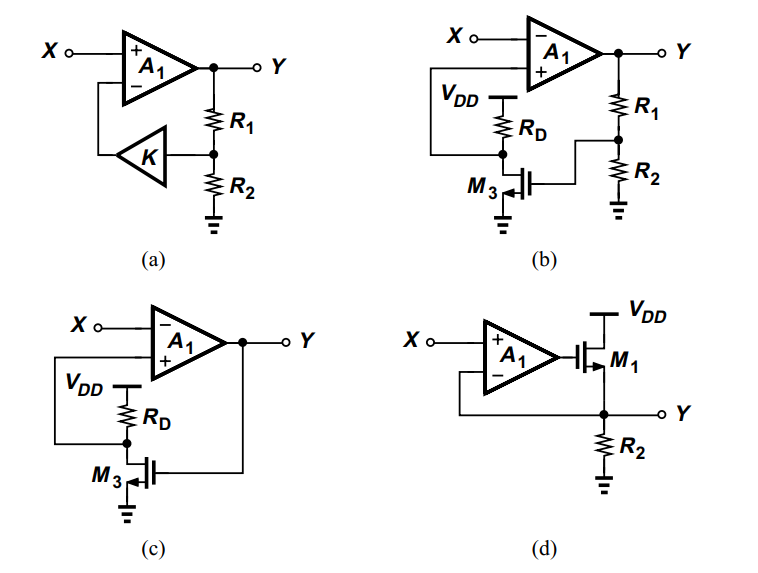
\includegraphics[width=0.505\textwidth]{p12-78.png}
        \caption*{Figure 12-78}
    \end{figure}        
\paragraph{解}
    \begin{figure}[!htb]
        \centering
        \begin{minipage}[t]{0.323\textwidth}
        \centering
        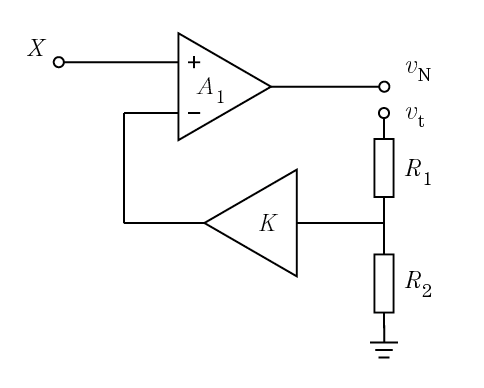
\includegraphics[width=1\textwidth]{p12-4-a.png}
        \caption*{(a)}
        \end{minipage}
        \begin{minipage}[t]{0.346\textwidth}
        \centering
        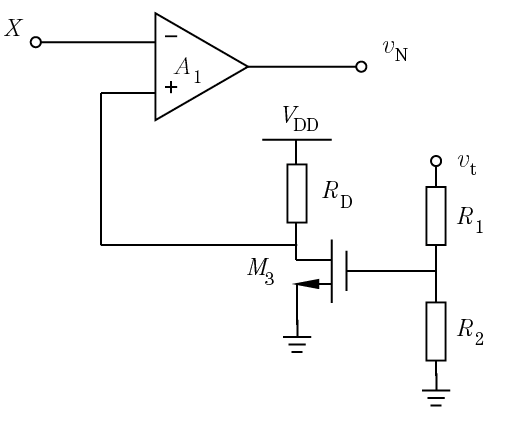
\includegraphics[width=1\textwidth]{p12-4-b.png}
        \caption*{(b)}
        \end{minipage}
        \\
        \begin{minipage}[t]{0.349\textwidth}
        \centering
        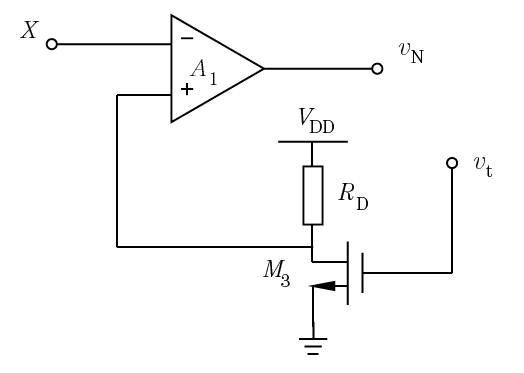
\includegraphics[width=1\textwidth]{p12-4-c.png}
        \caption*{(c)}
        \end{minipage}
        \begin{minipage}[t]{0.317\textwidth}
        \centering
        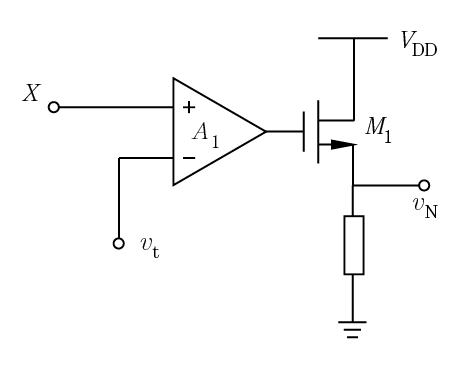
\includegraphics[width=1\textwidth]{p12-4-d.png}
        \caption*{(d)}
        \end{minipage}
        \caption*{Figure p12-4}
    \end{figure}    
    (a) 如图 p12-4-a,在$A_1$输出端断开环路。
    $$v_N = \frac{-R_2v_tKA_1}{R_1+R_2}$$
    则环路增益为$\frac{R_2KA_1}{R_1+R_2}$

    (b) 如图 p12-4-b,在$A_1$输出端断开环路。
    $$v_N = \frac{-R_2v_tg_{m3}R_DA_1}{R_1+R_2}$$
    则环路增益为$\frac{R_2g_{m3}R_DA_1}{R_1+R_2}$

    (c) 如图 p12-4-c,在$A_1$输出端断开环路。
    $$v_N = -v_tg_{m3}R_DA_1$$
    则环路增益为$g_{m3}R_DA_1$

    (d) 如图 p12-4-d,在$A_1$反相输入端断开环路。
    $$v_N = -v_tA_1 \cdot \frac{g_{m1}R_2}{1+g_{m1}R_2}$$
    则环路增益为$A_1 \cdot \frac{g_{m1}R_2}{1+g_{m1}R_2} \approx A_1$

\paragraph{12.5} \label{12.5}
    Using the results obtained in Problem 12.4, compute the closed-loop gain of the circuits shown in Fig. 12-78.
    \begin{figure}[!htb]
        \centering
        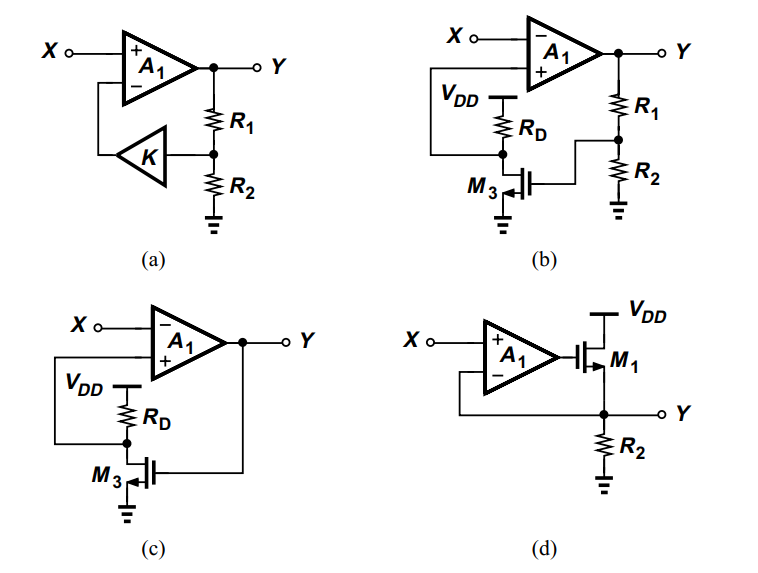
\includegraphics[width=0.505\textwidth]{p12-78.png}
        \caption*{Figure 12-78}
    \end{figure}        
\paragraph{解}
    (a) 
    $$A_{v,close} = \frac{A_1}{1+\frac{R_2KA_1}{R_1+R_2}}$$

    (b) 
    $$A_{v,close} = \frac{-A_1}{1 + \frac{R_2g_{m3}R_DA_1}{R_1+R_2}}$$

    (c)
    $$A_{v,close} = \frac{-A_1}{1 + g_{m3}R_DA_1}$$

    (d)
    $$A_{v,close} = \frac{-A_1g_{m1}R_2}{1+A_1 \cdot \frac{g_{m1}R_2}{1+g_{m1}R_2}} \approx \frac{-A_1g_{m1}R_2}{1+A_1}$$
\paragraph{12.10} \label{12.10}
    The circuit of Fig. 12-80 must achieve a closed-loop $-3\decibel$ bandwidth of $B$. Determine the required value of $K$. Neglect other capacitances and assume $\lambda > 0$.
    \begin{figure}[!htb]
        \centering
        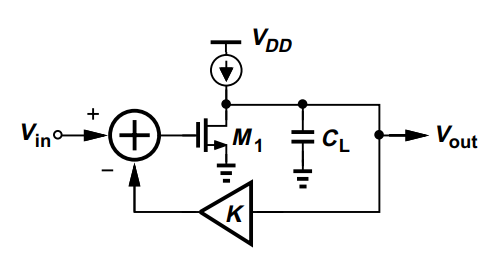
\includegraphics[width=0.325\textwidth]{p12-80.png}
        \caption*{Figure 12-80}
    \end{figure}        
\paragraph{解}
    \begin{align*}
        \omega_0 & = \under{C_Lr_{o1}} \\
        A_0 & = -g_{m1}r_{o1} 
    \end{align*}
    $$B = (1+|A_0|K)\omega_0$$ 
    $$\therefore K = \frac{C_Lr_{o1}B - 1}{g_{m1}r_{o1}}$$
\paragraph{12.22} \label{12.22}
    Determine the polarity of feedback in each of the stages illustrated in Fig. 12-87.
    \begin{figure}[!htb]
        \centering
        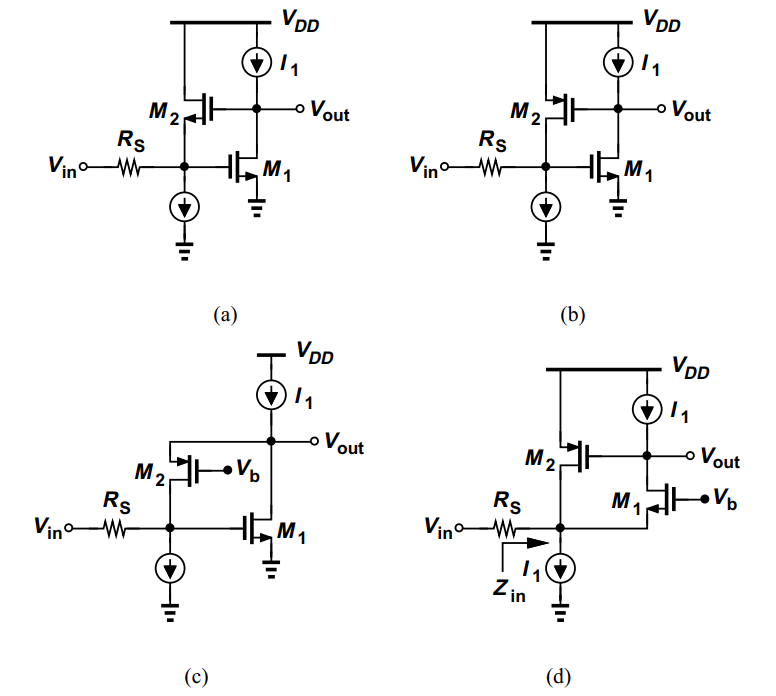
\includegraphics[width=0.517\textwidth]{p12-87.png}
        \caption*{Figure 12-87}
    \end{figure}        
\paragraph{解}
    (a) 设$M_1$栅端电压$V_1$上升,由$M_1$栅漏反极性可知$V_{out}$下降,又由$M_2$栅源同极性知$V_1$下降,从而为负反馈。
    
    (b) 设$M_1$栅端电压$V_1$上升,由$M_1$栅漏反极性可知$V_{out}$下降,又由$M_2$栅漏反极性知$V_1$上升,从而为正反馈。

    (c) 设$M_1$栅端电压$V_1$上升,由$M_1$栅漏反极性可知$V_{out}$下降,又由$M_2$源漏同极性知$V_1$下降,从而为负反馈。

    (d) 设$M_1$源端电压$V_1$上升,由$M_1$源漏同极性可知$V_{out}$上升,又由$M_2$栅漏反极性知$V_1$下降,从而为负反馈。

\paragraph{12.25} \label{12.25}
    Consider the feedback circuit shown in Fig. 12-88, where $R_1 + R_2 >> R_D$. Compute the closed-loop gaina and I/0 impedances of the circuit. Assume $\lambda \neq 0$.
    \begin{figure}[!htb]
        \centering
        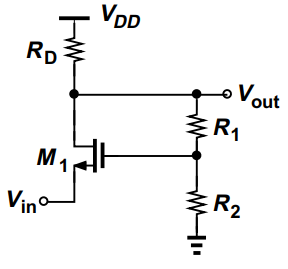
\includegraphics[width=0.192\textwidth]{p12-88.png}
        \caption*{Figure 12-88}
    \end{figure}        
\paragraph{解}
    \begin{align*}
        A_0 & = g_{m1}[R_D // (R_1+R_2) // r_{o1}] \approx g_{m1}(R_D // r_{o1}) \\
        K & = \frac{R_2}{R_1+R_2} \\
        R_{in} & = \under{g_{m1}} \\
        R_{out} & = R_D // (R_1+R_2) // r_{o1} \approx R_D // r_{o1} 
    \end{align*}
    \begin{align*}
        \therefore A_{v, close} & = \frac{g_{m1}(R_D // r_{o1})}{1+\frac{g_{m1}(R_D // r_{o1})R_2}{R_1+R_2}} \\
        R_{in,close} & = \under{g_{m1}}\left[1+\frac{g_{m1}(R_D // r_{o1})R_2}{R_1+R_2}\right] \\
        R_{out,close} & = \frac{R_D // r_{o1}}{1+\frac{g_{m1}(R_D // r_{o1})R_2}{R_1+R_2}}
    \end{align*}
\paragraph{12.33} \label{12.33}
    The amplifier depicted in Fig. 12-95 consists of a common-gate stage ($M_1$ and $R_D$) and a feedback network ($R_1, R_2$ and $M_2$). Assuming $R_1+R_2$ is very large and $\lambda = 0$, compute the closed-loop gain and I/O impedances.
    \begin{figure}[!htb]
        \centering
        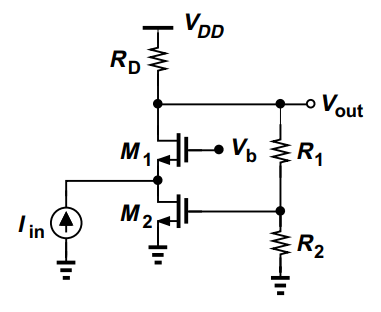
\includegraphics[width=0.254\textwidth]{p12-95.png}
        \caption*{Figure 12-95}
    \end{figure}        
\paragraph{解}
    \begin{align*}
        R_0 & = \under{g_{m1}} \cdot g_{m1}[R_D // (R_1+R_2)] \approx R_D\\
        K & = \frac{R_2g_{m2}}{R_1+R_2} \\
        R_{in} & = \under{g_{m1}} \\
        R_{out} & = R_D // (R_1+R_2) \approx R_D 
    \end{align*}
    \begin{align*}
        \therefore R_{v, close} & = \frac{R_D}{1+\frac{R_DR_2g_{m2}}{R_1+R_2}} \\
        R_{in,close} & = \under{g_{m1}\left(1+\frac{R_DR_2g_{m2}}{R_1+R_2}\right)} \\
        R_{out,close} & = \frac{R_D}{1+\frac{R_DR_2g_{m2}}{R_1+R_2}}
    \end{align*}
\paragraph{12.56} \label{12.56}
    Compute the closed-loop gain and I/O impedances of the stages illustrated in Fig. 12-117.
    \begin{figure}[!htb]
        \centering
        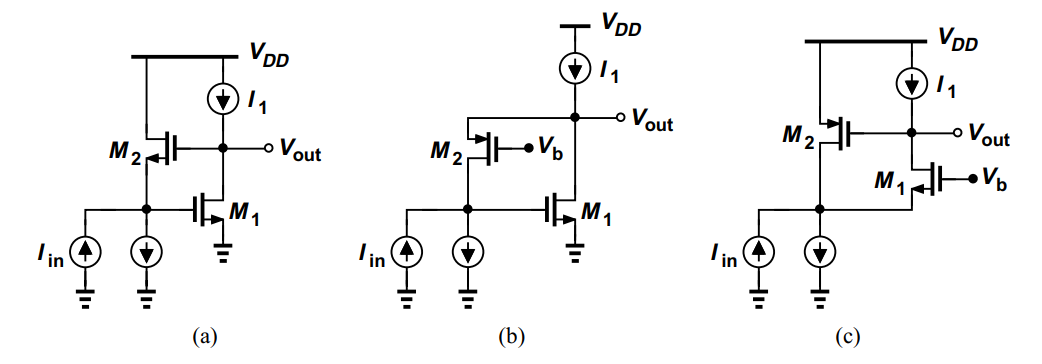
\includegraphics[width=0.695\textwidth]{p12-117.png}
        \caption*{Figure 12-117}
    \end{figure}        
\paragraph{解}
    (a) 视$M_2$为反馈部分。
    \begin{align*}
        R_{in} & = \under{g_{m2}} \\
        R_{out} & = r_{o1} // r_{o2} \\
        R_0 & = -\frac{g_{m1}}{g_{m2}}(r_{o1}//r_{o2})\\
        K & = g_{m2} \cdot \frac{g_{m2}r_{o2}}{1+g_{m2}r_{o2}} \approx g_{m2}
    \end{align*}
    \begin{align*}
        \therefore R_{v, close} & = \frac{-\frac{g_{m1}}{g_{m2}}(r_{o1}//r_{o2})}{1+g_{m1}(r_{o1}//r_{o2})} \\
        R_{in,close} & = \under{g_{m2}[1+g_{m1}(r_{o1}//r_{o2})]}\\
        R_{out,close} & = \frac{r_{o1}//r_{o2}}{1+g_{m1}(r_{o1}//r_{o2})}
    \end{align*}

    (b) 视$M_2$为反馈部分。
    \begin{align*}
        R_{in} & = r_{o2} \\
        R_{out} & = r_{o1} // \under{g_{m2}} \approx \under{g_{m2}} \\
        R_0 & = -r_{o1}g_{m1}(\under{g_{m2}}//r_{o1}) \approx -\frac{r_{o2}g_{m1}}{g_{m2}}\\
        K & = g_{m2}
    \end{align*}
    \begin{align*}
        \therefore R_{v, close} & = \frac{-r_{o2}g_{m1}}{g_{m2}(1+g_{m1}r_{o2})} \\
        R_{in,close} & = \frac{r_{o2}}{1+g_{m1}r_{o2}}\\
        R_{out,close} & = \under{g_{m2}(1+g_{m1}r_{o2})}
    \end{align*}

    (c) 视$M_2$为反馈部分。
    \begin{align*}
        R_{in} & = r_{o2} // \under{g_{m1}} \approx \under{g_{m1}} \\
        R_{out} & = r_{o1} \\
        R_0 & = \under{g_{m1}} \cdot g_{m1} r_{o1} = r_{o1} \\
        K & = -\under{g_{m1}} \cdot g_{m2}g_{m1} = -g_{m2}
    \end{align*}
    \begin{align*}
        \therefore R_{v, close} & = \frac{r_{o1}}{1+r_{o1}g_{m2}}\\
        R_{in,close} & = \under{(1+r_{o1}g_{m2})g_{m1}}\\
        R_{out,close} & = \frac{r_{o1}}{1+r_{o1}g_{m2}}
    \end{align*}
\end{document} 